% 图 2.11 L=3, S=3/2 角动量组合：上半 m_L-m_S 网格，下半按 J 分组的 m_J 态
\documentclass[tikz,border=5pt]{standalone}
\usetikzlibrary{arrows.meta}
\usepackage{amsmath}
\usepackage{bm}
\usepackage{fontspec}
\setmainfont{Times New Roman}
\begin{document}
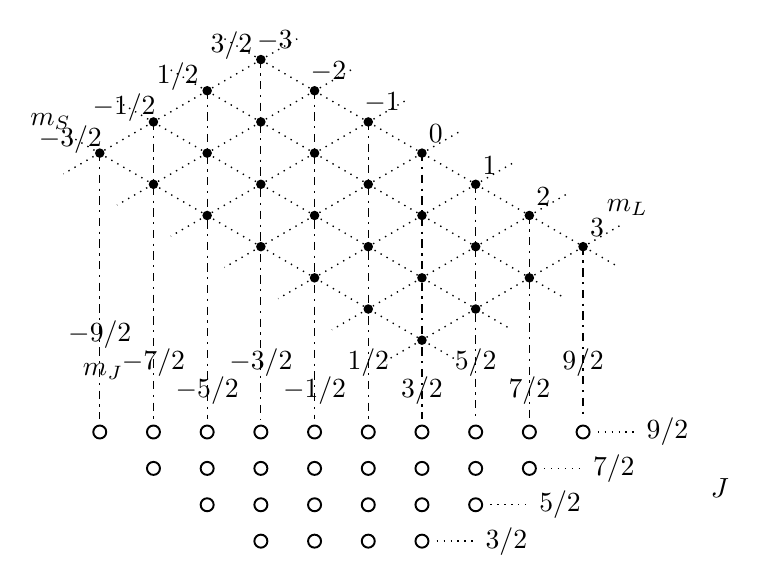
\begin{tikzpicture}[line width=0.8pt,>=Stealth,scale=1.1]
% 网格点： (m_L,m_S) -> (0.62(L+S+1.5), -0.36(L-S+4.5))
% 点阵
\foreach \L in {-3,-2,...,3}
  \foreach \S in {-1.5,-0.5,0.5,1.5}{
    \pgfmathsetmacro\x{0.62*(\L+\S+1.5)}
    \pgfmathsetmacro\y{-0.36*(\L-\S+4.5)}
    \fill (\x,\y) circle (0.055);
  }
% 点阵虚线（沿 u 与 w 两个方向，超出边界一点）
\foreach \S in {-1.5,-0.5,0.5,1.5}{
  \pgfmathsetmacro\xa{0.62*(-3+\S+1.5)-0.42}
  \pgfmathsetmacro\ya{-0.36*(-3-\S+4.5)+0.24}
  \pgfmathsetmacro\xb{0.62*(3+\S+1.5)+0.42}
  \pgfmathsetmacro\yb{-0.36*(3-\S+4.5)-0.24}
  \draw[dotted,line width=0.5pt] (\xa,\ya) -- (\xb,\yb);
}
\foreach \L in {-3,-2,...,3}{
  \pgfmathsetmacro\xc{0.62*(\L+3)+0.42}
  \pgfmathsetmacro\yc{-0.36*(\L+3)+0.24}
  \pgfmathsetmacro\xd{0.62*\L-0.42}
  \pgfmathsetmacro\yd{-0.36*(\L+6)-0.24}
  \draw[dotted,line width=0.5pt] (\xc,\yc) -- (\xd,\yd);
}
% 竖直点划线（从各列最高点落到圆点区顶部）
\foreach \M in {-4.5,-3.5,...,4.5}{
  \pgfmathsetmacro\xm{0.62*\M+0.93}
  \pgfmathsetmacro\yt{-0.36*abs(\M+1.5)}
  \draw[dash dot,line width=0.45pt] (\xm,\yt) -- (\xm,-4.15);
}
% m_J 轴标签（高低交错）
\foreach \M/\lab in {-4.5/{{$-9/2$}},-3.5/{{$-7/2$}},-2.5/{{$-5/2$}},-1.5/{{$-3/2$}},
  -0.5/{{$-1/2$}},0.5/{{$1/2$}},1.5/{{$3/2$}},2.5/{{$5/2$}},3.5/{{$7/2$}},4.5/{{$9/2$}}}{
  \pgfmathsetmacro\xm{0.62*\M+0.93}
  \pgfmathsetmacro\ylv{mod(\M+3.5,2)}
  \pgfmathsetmacro\ym{-3.5-0.32*\ylv}
  \node[inner sep=1pt] at (\xm,\ym) {\lab};
}
\node[anchor=east,inner sep=1pt] at (-1.55,-3.6) {$m_J$};
% 四行空心圆点（J=9/2,7/2,5/2,3/2），每行 2J+1 个
\foreach \J/\yR/\lab in {4.5/-4.3/{{$9/2$}},3.5/-4.72/{{$7/2$}},
  2.5/-5.14/{{$5/2$}},1.5/-5.56/{{$3/2$}}}{
  \foreach \M in {-4.5,-3.5,...,4.5}{
    \pgfmathsetmacro\keep{abs(\M)<=\J+0.01 ? 1 : 0}
    \ifnum\keep>0
      \pgfmathsetmacro\xm{0.62*\M+0.93}
      \draw[line width=0.7pt] (\xm,\yR) circle (0.075);
    \fi
  }
  \draw[dotted,line width=0.5pt] ({0.62*\J+1.10},\yR) -- ({0.62*\J+1.52},\yR);
  \node[anchor=west,inner sep=1pt] at ({0.62*\J+1.62},\yR) {\lab};
}
\node[anchor=west,inner sep=1pt] at (5.15,-4.95) {$J$};
% m_L 标签（沿右上边缘）
\foreach \L/\lab in {-3/{{$-3$}},-2/{{$-2$}},-1/{{$-1$}},0/{{$0$}},
  1/{{$1$}},2/{{$2$}},3/{{$3$}}}{
  \node[inner sep=1pt] at ({0.62*(\L+3)+0.16},{-0.36*(\L+3)+0.22}) {\lab};
}
\node[anchor=south west,inner sep=1pt] at (3.95,-1.85) {$m_L$};
% m_S 标签（沿左上边缘）
\foreach \S/\lab in {1.5/{{$3/2$}},0.5/{{$1/2$}},-0.5/{{$-1/2$}},-1.5/{{$-3/2$}}}{
  \node[inner sep=1pt] at ({0.62*(\S-1.5)-0.34},{-0.36*(1.5-\S)+0.16}) {\lab};
}
\node[anchor=east,inner sep=1pt] at (-2.15,-0.72) {$m_S$};
\end{tikzpicture}
\end{document}
